%
% FH Technikum Wien
% !TEX encoding = UTF-8 Unicode
%
% Erstellung von Master- und Bachelorarbeiten an der FH Technikum Wien mit Hilfe von LaTeX und der Klasse TWBOOK
%
% Um ein eigenes Dokument zu erstellen, müssen Sie folgendes ergänzen:
% 1) Mit \documentclass[..] einstellen: Master- oder Bachelorarbeit, Studiengang und Sprache
% 2) Mit \newcommand{\FHTWCitationType}.. Zitierstandard festlegen (wird in der Regel vom Studiengang vorgegeben - bitte erfragen)
% 3) Deckblatt, Kurzfassung, etc. ausfüllen
% 4) und die Arbeit schreiben (die verwendeten Literaturquellen in Literatur.bib eintragen)
%
% Getestet mit TeXstudio mit Zeichenkodierung ISO-8859-1 (=ansinew/latin1) und MikTex unter Windows
% Zu beachten ist, dass die Kodierung der Datei mit der Kodierung des paketes inputenc zusammen passt!
% Die Kodierung der Datei twbook.cls MUSS ANSI betragen!
% Bei der Verwendung von UTF8 muss dnicht nur die Kodierung des Dokuments auf UTF8 gestellt sein, sondern auch die des BibTex-Files!
%
% Bugreports und Feedback bitte per E-Mail an latex@technikum-wien.at
%
% Versionen
% *) V0.7: 9.1.2015, RO: Modeline angepasst und verschoben
% *) V0.6: 10.10.2014, RO: Weitere Anpassung an die UK
% *) V0.5: 8.8.2014, WK: Literaturquellen überarbeitet und angepasst
% *) V0.4: 4.8.2014, WK: Initalversion in SVN eingespielt
%
\documentclass[Bachelor,BIF,english]{twbook}
\usepackage[utf8]{inputenc}
\usepackage[T1]{fontenc}

%
% Bitte in der folgenden Zeile den Zitierstandard festlegen
\newcommand{\FHTWCitationType}{IEEE} % IEEE oder HARVARD möglich - wenn Sie zwischen IEEE und HARVARD wechseln, bitte die temorären Dateien (aux, bbl, ...) löschen
%
\ifthenelse{\equal{\FHTWCitationType}{HARVARD}}{\usepackage{harvard}}{\usepackage{bibgerm}}

% Definition Code-Listings Formatierung:
\usepackage[final]{listings}
\lstset{captionpos=b, numberbychapter=false,caption=\lstname,frame=single, numbers=left, stepnumber=1, numbersep=2pt, xleftmargin=15pt, framexleftmargin=15pt, numberstyle=\tiny, tabsize=3, columns=fixed, basicstyle={\fontfamily{pcr}\selectfont\footnotesize}, keywordstyle=\bfseries, commentstyle={\color[gray]{0.33}\itshape}, stringstyle=\color[gray]{0.25}, breaklines, breakatwhitespace, breakautoindent}
\lstloadlanguages{[ANSI]C, C++, [gnu]make, gnuplot, Matlab}

%Formatieren des Quellcodeverzeichnisses
\makeatletter
% Setzen der Bezeichnungen für das Quellcodeverzeichnis/Abkürzungsverzeichnis in Abhängigkeit von der eingestellten Sprache
\providecommand\listacroname{}
\@ifclasswith{twbook}{english}
{%
    \renewcommand\lstlistingname{Code}
    \renewcommand\lstlistlistingname{List of Code}
    \renewcommand\listacroname{List of Abbreviations}
}{%
    \renewcommand\lstlistingname{Quellcode}
    \renewcommand\lstlistlistingname{Quellcodeverzeichnis}
    \renewcommand\listacroname{Abkürzungsverzeichnis}
}
% Wenn die Option listof=entryprefix gewählt wurde, Definition des Entyprefixes für das Quellcodeverzeichnis. Definition des Macros listoflolentryname analog zu listoflofentryname und listoflotentryname der KOMA-Klasse
\@ifclasswith{scrbook}{listof=entryprefix}
{%
    \newcommand\listoflolentryname\lstlistingname
}{%
}
\makeatother
\newcommand{\listofcode}{\phantomsection\lstlistoflistings}

% Die nachfolgenden Pakete stellen sonst nicht benötigte Features zur Verfügung
\usepackage{blindtext}
\usepackage{parskip}
\usepackage{epstopdf}

\hyphenchar\font=\string"7F
\hyphenation{TESTS-Name-Of-Browser-Version-Of-Browser-Name-Of-Operating-System-Version-Of-Operating-System-xml}

%
% Einträge für Deckblatt, Kurzfassung, etc.
%
\title{Rebuilding a SharePoint 2013 Application with Angular 7 and Reactive Programming}
\author{Dominik Hack}
\studentnumber{1610257044}
\supervisor{DI Thomas Rongitsch}
\place{Vienna}
\kurzfassung{text}
\schlagworte{schlagwort1}
\outline{text}
\keywords{keyword1}

\begin{document}

%Festlegungen für den HARVARD-Zitierstandard
\ifthenelse{\equal{\FHTWCitationType}{HARVARD}}{
\bibliographystyle{Harvard_FHTW_MR}%Zitierstandard FH Technikum Wien, Studiengang Mechatronik/Robotik, Version 1.2e
\citationstyle{dcu}%Correct citation-style (Harvardand, ";" between citations, "," between author and year)
\citationmode{abbr}%use "et al." with first citation
\iflanguage{ngerman}{
    %Deutsch Neue Rechtschreibung
    \newcommand{\citepic}[1]{(Quelle: \protect\cite{#1})}%Zitat: Bild
    \newcommand{\citefig}[2]{(Quelle: \protect\cite{#1}, S. #2)}%Zitat: Bild aus Dokument
    \newcommand{\citefigm}[2]{(Quelle: modifiziert "ubernommen aus \protect\cite{#1}, S. #2)}%Zitat: modifiziertes Bild aus Dokument
    \newcommand{\citep}{\citeasnoun}%In-Line Zitiat entweder mit \citep{} oder \citeasnoun{}
    \newcommand{\acessedthrough}{Verf{\"u}gbar unter:}%Für URL-Angabe
    \newcommand{\acessedthroughp}{Verf{\"u}gbar bei:}%Für URL-Angabe (Geschützte Datenbank, Zugriff durch FH)
    \newcommand{\acessedat}{Zugang am}%Für URL-Datum-Angabe
    \newcommand{\singlepage}{S.}%Für Seitenangabe (einzelne Seite)
    \newcommand{\multiplepages}{S.}%Für Seitenangabe (mehrere Seiten)
    \newcommand{\chapternr}{K.}%Für Kapitelangabe
    \renewcommand{\harvardand}{\&}%Harvardand in Zitaten
    \newcommand{\abstractonly}{ausschließlich Abstract}
    \newcommand{\edition}{. Auflage}%Angabe der Auflage
}{
\iflanguage{german}{
    %Deutsch
    \newcommand{\citepic}[1]{(Quelle: \protect\cite{#1})}%Zitat: Bild
    \newcommand{\citefig}[2]{(Quelle: \protect\cite{#1}, S. #2)}%Zitat: Bild aus Dokument
    \newcommand{\citefigm}[2]{(Quelle: modifiziert "ubernommen aus \protect\cite{#1}, S. #2)}%Zitat: modifiziertes Bild aus Dokument
    \newcommand{\citep}{\citeasnoun}%In-Line Zitiat entweder mit \citep{} oder \citeasnoun{}
    \newcommand{\acessedthrough}{Verf{\"u}gbar unter:}%Für URL-Angabe
    \newcommand{\acessedthroughp}{Verf{\"u}gbar bei:}%Für URL-Angabe (Geschützte Datenbank, Zugriff durch FH)
    \newcommand{\acessedat}{Zugang am}%Für URL-Datum-Angabe
    \newcommand{\singlepage}{S.}%Für Seitenangabe (einzelne Seite)
    \newcommand{\multiplepages}{S.}%Für Seitenangabe (mehrere Seiten)
    \newcommand{\chapternr}{K.}%Für Kapitelangabe
    \renewcommand{\harvardand}{\&}%Harvardand in Zitaten
    \newcommand{\abstractonly}{ausschließlich Abstract}
    \newcommand{\edition}{. Auflage}%Angabe der Auflage
}{
    %Englisch
    \newcommand{\citepic}[1]{(Source: \protect\cite{#1})}%Zitat: Bild
    \newcommand{\citefig}[2]{(Source: \protect\cite{#1}, p. #2)}%Zitat: Bild aus Dokument
    \newcommand{\citefigm}[2]{(Source: taken with modification from \protect\cite{#1}, p. #2)}%Zitat: modifiziertes Bild aus Dokument
    \newcommand{\citep}{\citeasnoun}%In-Line Zitiat entweder mit \citep{} oder \citeasnoun{}
    \newcommand{\acessedthrough}{Available at:}%Für URL-Angabe
    \newcommand{\acessedthroughp}{Available through:}%Für URL-Angabe (Geschützte Datenbank, Zugriff durch FH)
    \newcommand{\acessedat}{Accessed}%Für URL-Datum-Angabe
    \newcommand{\singlepage}{p.}%Für Seitenangabe (einzelne Seite)
    \newcommand{\multiplepages}{pp.}%Für Seitenangabe (mehrere Seiten)
    \newcommand{\chapternr}{Ch.}%Für Kapitelangabe
    \renewcommand{\harvardand}{\&}%Harvardand in Zitaten
    \newcommand{\abstractonly}{Abstract only}
    \newcommand{\edition}{~edition}%Edition -> note, that you have to write "edition = {2nd},"!
}}}

\maketitle
\chapter{Introduction}
describe starting point, why will this project be realised, what should be achieved?, motivation, SharePoint \cite{SharePoint}, SharePoint Requirements (IE), Project Requirements (features), old solution, rebuilding with angular because of new features and same cost of developing a new application and not building on sharepoint feature (also extensibility, maintenance and encapsulation), better for company to have knowledge in Angular than in Sharepoint 2013 (because more projects also use angular), possible research questions: extensibility (1 of 4 team members have experience in developing sharepoint apps, 3 of 4 team members have experience in developing angular apps), maintenance?, observer patter in reactive programming?, overhead of redux?, war angular wirklich schneller zu entwickeln als sharepoint? (Vorteile: Angular wird häufig auch bei anderen Projekten verwendet, no publishing of whole sharepoint project through hosting angular app locally which saves time also angular supports hot reloading)
\clearpage


\chapter{Tools \& Frameworks} 
what will be presented in this chapter (reactive programming; tools to use this paradigm with: ReactiveX, Redux and NgRx; Angular; why typescript; what components are; introduction of important tools used by angular: npm, webpack and babel),
For the implementation of this project a technology had to be decided on that meets the requirements of being integrated into and communicate with SharePoint 2013.

\section{Reactive Programming}
If an interaction with a reactive application takes place, a event occurs which the software will respond on by reacting on it in a certain way. Therefore a reactive software system could be any application with a graphical user interface (GUI) reacting on user input, a network monitoring service reacting on certain changes of the network or even a simple calculator reacting on button presses. reactive applications can become complex because of a mixed combination of data and control flow \cite[p.~1]{PositivEffectOfRP}, 
two main approaches to implement a reactive application (also explain figure):
\begin{figure}[!htbp]
\centering
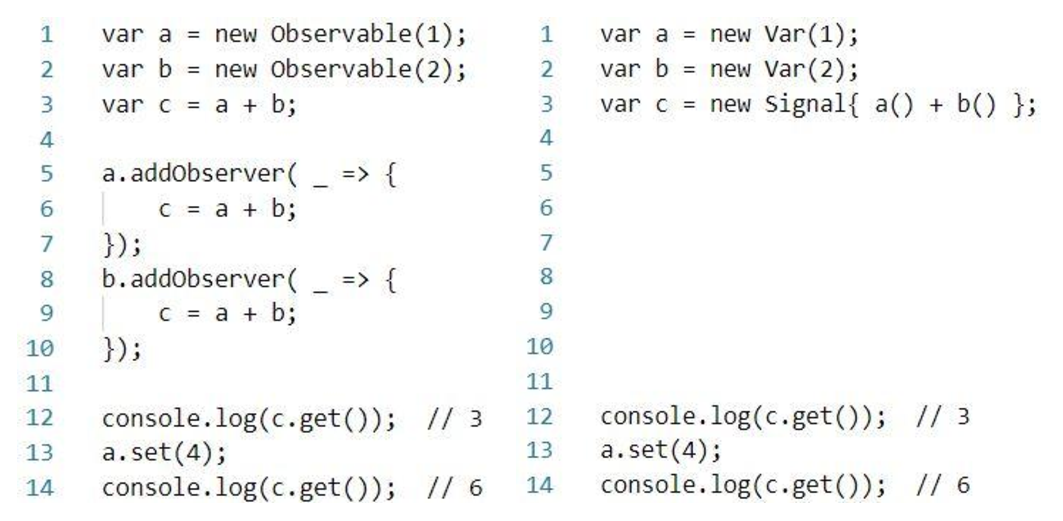
\includegraphics[width=0.75\linewidth]{PICs/pseudo_Code_reactive_2_ways.eps}
\caption{JavaScript-like pseudo code of the observer pattern approach (left) and the signals and vars approach (right) \cite[p.~797]{DebuggingRP} \cite[p.~3]{PositivEffectOfRP}}\label{Fig1}
\end{figure}
traditional approach observer pattern \cite[p.~360-372]{ObserverDP}, decouples event consumers from event producers \cite[p.~953]{RPWalkthrough}, (in object oriented programming using observer pattern, decouples observers or subscribers from observables or subjects, observers subscribe to observables, observables do not know their subscribers, when observables change their state they notify their observers depending on the implementation this can be done through emitting events. When a subscriber learns of a change in the state of the subject, he adjusts his state to that of the subject. \cite[p.~363]{ObserverDP}),
vs the other way, what is reactive programming: programming paradigm supporting language-level abstractions \cite[p.~953]{RPWalkthrough}, The four principles all implementations of reactive programming pursue are:
\begin{itemize}
\item Declarativeness: declaring how the states of the components depend on each other, not how to retrieve the state when changes occur \cite[p.~2]{PositivEffectOfRP}.
\item Abstraction over change propagation: No need to manually update dependencies, propagation of change is handled by language runtime \cite[p.~2]{PositivEffectOfRP}.
\item Composability: Composing reactive computations through abstractions \cite[p.~2]{PositivEffectOfRP}.
\item Favoring data flow over control flow: Calculations of the software system are triggered by new data or events and are not depending on the execution of the control flow \cite[p.~2]{PositivEffectOfRP}.
\end{itemize}
einiges an Forschung wurde schon betrieben und nach der Einführung von funcitonal reactive programming in Haskell wurde dieses konzept auch in Scheme (FrTime \cite{FrTime}), Scala (Scala.react \cite{DeprecatingOP}) und JavaScript (Flapjax \cite{Flapjax}) implementiert, sogar wurde in Microsofts Reactive Extensions (RX or ReactiveX) konzepte von reactive programming implementiert \cite[p.~954]{RPWalkthrough} \cite[p.~796]{DebuggingRP} \cite[p.~2]{PositivEffectOfRP}
(signals or behaviours: time changing values, treated as constraints of the language runtime, when an inconcistency of a signal or behaviour is detected a recalculation is triggered \cite[p.~797]{DebuggingRP} \cite[p.~3]{PositivEffectOfRP}, can either depend on other signals or vars, vars are reactive values like signals but without dependencies \cite[p.~2]{PositivEffectOfRP}), less error prone, easier to understand, still immature field -> lack of developer tools like debuggers \cite[p.~796]{DebuggingRP}

\subsection{ReactiveX}
general introduction (what is it \cite{ReactiveExtensions} (von Microsoft aber open source), why should it be used) \cite{ReactiveX}, bringing functional-reactive-programming-like reactivity (FRP-like reactivity), 
marble-diagrams
\begin{figure}[!htbp]
\centering
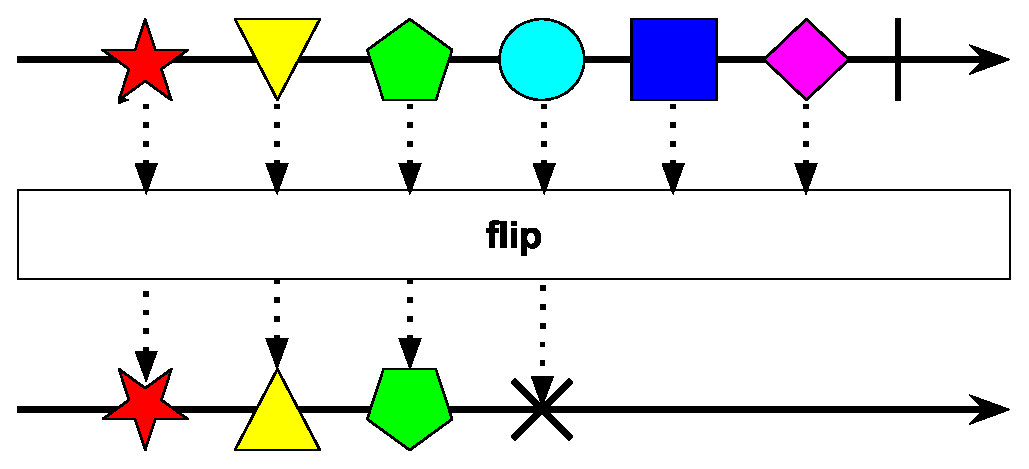
\includegraphics[width=0.5\linewidth]{PICs/marble_diagram.eps}
\caption{An example of a marble diagram, which is mostly used for explaining transformations of observables \cite{RxObservables}.}\label{Fig2}
\end{figure}
observables, observables background with reactor pattern \cite{RxObservables}

\subsection{Redux}
general introduction (what is it, why should it be used), \cite{Redux}, motivation why redux \cite{ReduxIntroMoti}, core concept \cite{ReduxIntroCC}, three principles \cite{ReduxIntro3P}, figure for explanation

\subsection{NgRx}
general introduction (what is it, why should it be used), \cite{Ngrx}, ng/store, effects


\section{Angular}
what is angular?, what is it for?, dependency injection, data binding, \cite[p.~]{YakovFainAngular}

\subsection{TypeScript}
general introduction (what is it, why should it be used), 

\subsection{Components}
general introduction (what is it, why should it be used, structured inside of a module), 

\subsection{npm}
general introduction (what is it, why should it be used), 
tool to install everything js based

\subsection{Webpack}
general introduction (what is it, why should it be used), 
bundling assets (vendor, main, styles, etc.)

\subsection{Babel}
general introduction (what is it, why should it be used), 
polyfills

\clearpage 

\chapter{Implementation}
The following sections deal with describing the processes utilized to ensure the quality of the final product both during the development phase and after completion. First, the general procedures related to project management and continuous integration are illustrated. Subsequently, the software architecture including the project structure, the interfaces and additionally added technologies as well as methodologies will be presented. Finally, the development with reactive programming is discussed.

\section{Project Management}
To successfully complete this project with as few errors as possible and to develop a product that adds business value to the customer and satisfies the customers' needs, the agile project management framework "Scrum" \cite{Scrum} was employed. The scrum team consisted of 3 developers, one of whom was one half of his time involved in scrum master activities, and one product owner. The product owner took care of analyzing the current problems together with the customer in order to develop a possible solution. Based on these requirements, a first version of the backlog was created to give the development team an overview of the product to be developed. Subsequently, the developer team estimated the story points of each user story using planning poker. With this information the product owner calculated the offer for the customer. After the contract was signed the scrum team met for a project kick-off meeting to discuss the highest priority user stories and refine the backlog for the first sprint.
\\[\baselineskip]
The length of a sprint for this project was one week, since at first the user stories were small enough so that the commitment to the sprint goal could be kept. Later, the length of a sprint was increased to two weeks, because on the one hand some user stories were too large to finish in a week and on the other hand a developer had to be assigned to other projects for some time. Sprints were planned using the user-story- and task-board-backlog tools provided by the company's TFS (Team Foundation Server) \cite{TFS}. After each sprint a short retro was held on the day of the planning where the finished user stories and the problems encountered while implementing them were deliberated. In addition when it occurred that a commitment could not be kept, the reasons were sought to make adjustments to user stories that could be affected. 
\\[\baselineskip]
Every day a daily stand-up was held where each developer announced the current status of their to them assigned user stories. If there was any difficulty implementing a user story, after the meeting, the task in question was discussed with at least one other developer. If no solution was found, the product owner was contacted to discuss the problem. This led in most cases to an adaptation of the acceptance criteria of the user story, only rarely the customer had to be contacted to discuss the respective requirement. 
\\[\baselineskip]
If all tasks of a user story were implemented and thus also fulfilled all acceptance criteria, the user story could be closed and a pull request could be created. The pull request was accepted when another developer agreed to the changes and the build process, which is described in more detail in the next chapter, succeeded. So that a user story was now considered as resolved, the product owner together with the developer tested the respective features on the development server. If changes still had to be made, the user story was set to active as long as there was still enough time in the running sprint otherwise it was put back in the backlog to be scheduled for the next sprint. After a certain number of user stories were resolved, a milestone was reached, meaning that a demo meeting with the customer was arranged in order to present the current status of the product. As a result, the current application was deployed on the user acceptance test server and then an in-house demo meeting with the scrum team was held to prepare and practice for the upcoming demo meeting with the customer. The feedback given by the customer during the demo meeting was collected by the product owner, who then adjusted the remaining user stories accordingly. If necessary, new user stories were created and added to the backlog. When all the user stories were resolved, a final demo meeting was held with the client, and after the final adjustments were integrated, the product was deployed to the client's production systems.

\section{Continuous Integration}
In order to detect as many bugs as possible before merging the changes with the master branch of the git \cite{Git} repository and maximizing the quality of the source code as well as the project structure, the development team defined a CI process with specific rules for the project. These rules applied to handling the local cloned git repository and when changes to the source code were accepted for merging with the shared repository. 
\\[\baselineskip]
Before starting the implementation of a user story, a feature branch had to be created, because committing on the master branch was not possible due to constraints and after merging the changes into the master branch, the respective branch had to be deleted. If the acceptance criteria of the user story were met, all changes to the source code had to be pushed to the shared repository and a pull request had to be created using the TFS user interface. The pull request was accepted if at least one other developer agreed, no comments on the source code were still marked as active, and the, on creation of the pull request automatically triggered, build process had been successfully completed. The review of the source code of the pull request was carried out by a code review with at least one other developer. If changes had to be made to the code after the code review, the pull request remained open. Only when all conditions had been fulfilled the pull request was completed.
\\[\baselineskip]
The build pipeline was designed utilizing the build definition user interface of the TFS \cite{TFSBuildPipeline} . The requirements for a build server for this procedure are that it has npm installed and has enough space to download and install the node modules. The build process consists of six tasks which are the following:
\begin{itemize}
\item "Get sources": As the name implies, this build step is responsible for getting the latest source code. When configuring the task, the name of the project, the name of the code repository as well as the name of the branch that should be fetched, after the process started, had to be defined.
\item "npm install": This step executes the command "npm install" and thus installs all required dependencies of the application which are defined in the "package-lock.json" file \cite{NpmInstall}. In the configuration of the step, the folder in which the "package.json" is located was specified, as this allows the task to keep in mind the additional configurations for the particular command to be executed \cite{NpmTaskInstall}.
\item "npm build": The use of this step is it to start a production build process. A custom command must be specified for this step because the build definition tool of the companies TFS did not support the command "npm run build" out of the box and furthermore additional arguments for the command had to be specified. The command that is executed is "npm run prod-build" which is an abbreviation for "ng build --prod --output-path='dist/blog-app'" defined in the "package.json" file. The argument "--prod" sets the production-flag to true and thereby executes a build which does not only employ bundeling and limited tree-shaking but also limited dead code elimination. The argument "--output-path" specifies the relative path to the folder where the compiled project will be moved \cite{AngularCliBuild}. As with the previous step, the folder in which the "package.json" file is located was specified \cite{NpmTaskCustom}.
\item "npm test": In this step, the test process is initiated. For the same reason as with the "npm build" step a custom command has to be configured. The command specified here is "npm run test-headless" which in turn is a short for "ng test --watch=false --browsers=PhantomJS --reporters=progress,junit". The argument "--watch=false" ensures that the test process is terminated after a run. The other two arguments define which reporter or browser should be operated by karma \cite{KarmaConfig}. As a reporter Progress and JUnit \cite{JUnit} \cite{KarmaJUnitReporter} were chosen, because firstly the test results generated by the Progress reporter can be found in the console output of the build job in the TFS and secondly a more pleasant view of the test results is generated by the TFS in the next step by interpreting the XML output of the test results created by the JUnit reporter. The reason why PhantomJS \cite{PhantomJS} was chosen as the browser in which the tests are running will be explained in the next paragraphs. As with the other two steps before, the folder in which the "package.json" file is was specified again \cite{NpmTaskCustom}.
\item "Publish Test Results": The test results created by the previous task are captured by this task and passed to the TFS in the correct format. The configuration of this build step consists of the respective format of the test results, the name of the file in which the test results are to be found and in which folder this file should be searched for. The name of the output file of the JUnit reporter is, unless the default configuration inside of the karma configuration file is changed, in the pattern "TESTS-Name-Of-Browser{\_}Version-Of-Browser{\_}(Name-Of-Operating-System{\_}Version-Of-Ope-\\rating-System).xml", therefore "TESTS-*.xml", where "*" serves as a wildcard, was set \cite{KarmaJUnitReporterConfig}. The default value "\$(System.DefaultWorkingDirectory)" for the search folder was retained because no changes were made to the configuration of the output folder of the JUnit Reporter \cite{TFSPublishBuildArtifact}.
\item "Publish Artifact: dist": In the last step, the files created by the build task are issued as artifacts. For this, the path to the folder containing the compiled files and the name of the artifact had to be specified. The value for the path was the output folder specified in the "--output-path" argument of the "npm build" command. For the name of the artifact "drop" was selected because it was a rule of the development team for this project to call each build artifact "drop". An artifact created by this task could be downloaded to manually deploy on a SharePoint 2013 development server or User Acceptance Test Server for further testing by a developer, the product owner or the customer \cite{TFSPublishBuildArtifact}.
\end{itemize}
For this project, the first build process for an Angular project of the development team has been created, which in addition to building the application also runs the tests and then publishes the results. This was mostly because the build servers had problems launching a browser like Google Chrome \cite{Chrome} or Mozilla Firefox \cite{Firefox} however, a browser is needed to run the tests with Karma as the test runner. The solution to this problem was to use a headless browser \cite[p.~2]{HeadlessBrowser} for executing the tests. In contrast to browsers like Google Chrome or Mozilla Firefox, headless browsers are always executed in the background and do not have a graphical user interface. The communication with a headless browser thus only takes place via the console, which allows a build server to run it. The selected headless browser for this project was PhantomJS \cite{PhantomJS}, as two developers of the team had already gained experience with PhantomJS.
\\[\baselineskip]
\begin{figure}[!htbp]
\centering
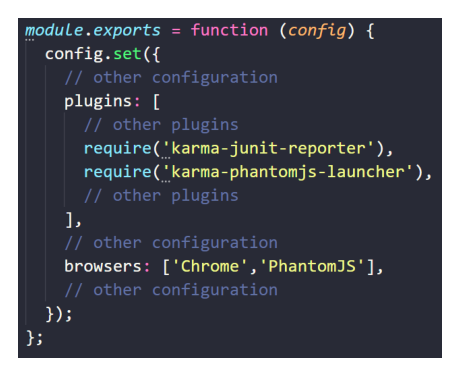
\includegraphics[width=0.5\linewidth]{PICs/karma_phantomjs.eps}
\caption{The "karma.conf.json" file with the configuration to utilize PhantomJS added to it}\label{Fig3}
\end{figure}
For PhantomJS to be operated as a browser for the test task, the three npm packages: phantomjs-prebuilt, karma-phantomjs-launcher, and karma-junit-reporter had to be included in the project and added to the karma configuration file as shown in the figure \ref{Fig3}. These packages install PhantomJs and two karma plugins, which allows Karma to run the tests inside of PhantomJS and create reports of the results which the TFS user interface can interpret and showcase. Additionally, a process variable with the value "C:/NPM/Modules/PhantomJS.cmd" had to be added to the build process, so that the respective agent finds the executable file of PhantomJS.

\section{Integrating Angular in SharePoint 2013}
In order to use Angular as the framework for developing the application, it was first necessary to find a way to host the application in SharePoint 2013. This problem was solved by injecting the compiled project files each inside of one HTML script tag into the script-editor-web-part of the landing page. For the value of the  HTML script tag's source attribute the path to the compiled files and for the value of the type attribute "text/javascript" was defined. As a result, when the page was loaded, the scripts were executed and thereby started the application. An advantage of this solution was that every developer could work locally on the blog application because the path to the compiled project files could also point to the output of the build process of the local server hosted by the Angular "ng serve"-command.
\\[\baselineskip]
However, one requirement of the development team was not having to think about the script editor web part of the blog application every time the project maintenance was released, which is why it was decided to develop a SharePoint feature \cite{SPFeature} and feature event receiver \cite{SPFeatureEventReceiver}. Furthermore a feature event receiver also solved the question how the data of the old blog application could be migrated automatically.
\\[\baselineskip]
A SharePoint feature, as the name suggests, offers further functionality and can be activated at any time by a user with high enough privileges. A feature event receiver waits until a feature related event shows up to respond to it. Such an event appears when activating, deactivating, installing or deleting a feature. One limitation that has been set up so that elements of the blog feature are not unnecessarily created on the entire system is that the developed feature can only be activated on pages where blogs have already been created. By activating the blog feature, the blog event receiver starts creating all the necessary elements and migrating the data from the old blog. The tasks of the blog event receiver are the following:
production integration uses paths to files compiled with a production build
feature receiver (migrates all configured settings, created content and subscribed alerts; ensures the creation of the page library, the landing page of the blog containing the script editor webpart to display the blog), 
\begin{itemize}
\item "MigrateBlog":
\item "EnsurePageLib":
\item "EnsureLandingPage":
\item "EnsureCategoryListFields":
\item "EnsureTagsList":
\item "EnsureBlogListFields":
\item "EnsureCategoryItemEventReceiver":
\item "EnsureTagsItemEventReceiver":
\item "ReorderFields":
\item "EnsureAlertManagerGroup":
\end{itemize}
polyfills have to be imported so application also works on Internet Explorer

\section{Software Architecture}

\subsection{Software Components}
created with angular-cli \cite{AngularCli};
core (grundgerüst der anwendung), blog, alert, shared, entities, services,
\\[\baselineskip]
service entities, containers, components, routing (router, guard);
\\[\baselineskip]
(über index.html direkt zur "app"-komponente welche dann wenn kein Fehler beim Laden des derzeitgen Users geworfen wird direkt mittels einer "router-outlet"-direktive auf den angegebenen Pfad weiterleitet. Wenn ein kein User eingeloggt ist oder dieser nicht berechtigt ist den Blog zu lesen wird eine Fehlerseite angezeigt und die jeweilige Fehlermeldung ausgegeben. wenn kein richtiger pfad dann auf "/blog" weitergeletitet, beim ansurfen ohne URL im Browser explizit angegeben zu haben wird auch auf "/blog" als Default verwiesen), ("blog-details"-guard überprüft nochmal ob ein User eingeloggt ist und berechtigt ist auf den Blog zuzugreifen bevor auf die Liste der Blogs weitergeleitet wird. jz sind wir in der applikation)

\subsection{Interfaces}
Principally, the developed application needs to communicate with only one other system, which is SharePoint 2013, but with which SharePoint interface has to be spoken changes, depending on where the data is requested from and what the demanded data is.
pnpjs \cite{Pnpjs} easier communication with SharePoint (requires a setup function to be executed in the "main.ts" file which defines all accepted headers of the requests and responses), 
JSOM und CSOM "sp" \cite{PnpjsSp} the fluent api wenn pnpjs verwendet werden kann, 
selbstgebautes Backend "REST" API mit Angulars "HttpClient",
SharePointHttpClient wenn extra Authenfizierung benötigt ist um Daten zu beanspruchen,
SharePoint Script On Demand

\subsection{Styles}
SCSS, BEM

\section{Reactive Programming}

\subsection{Libraries \& Development Tools}
rxjs,
\\[\baselineskip]
\begin{figure}[!htbp]
\centering
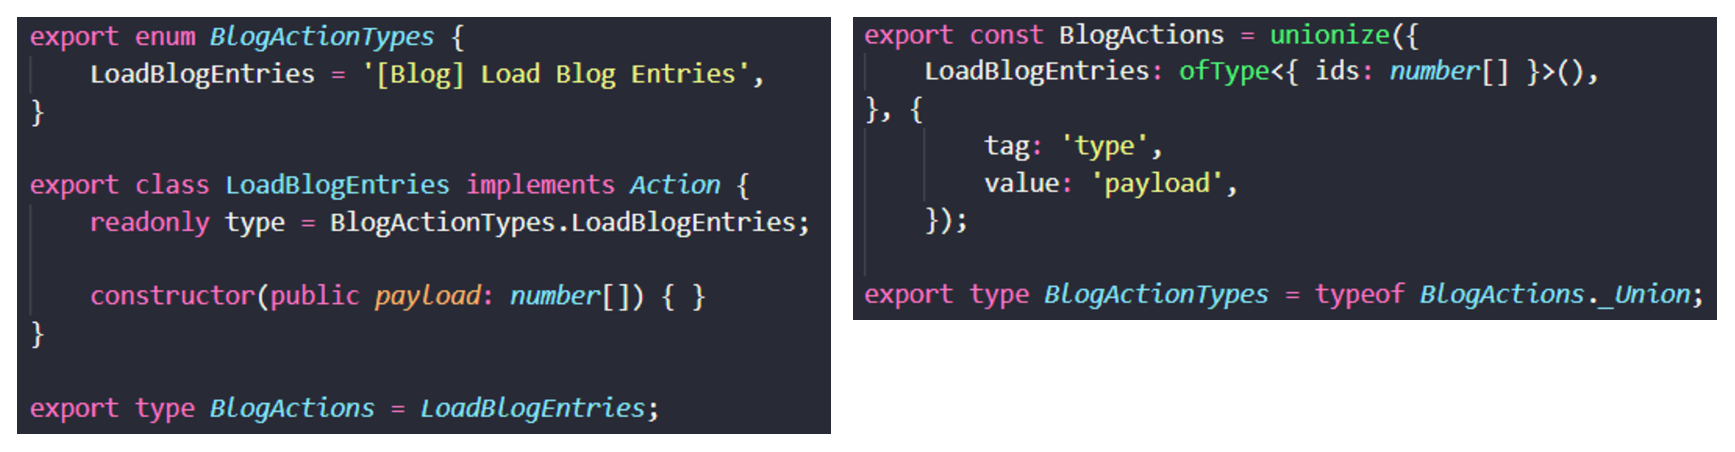
\includegraphics[width=1\linewidth]{PICs/without_and_with_unionize_actions.eps}
\caption{"LoadBlogEntriesAction" implemented without (left) and with the use of the methods "unionize" and "ofType" from the TypeScript library Unionize \cite{Unionize} (right).}\label{Fig4}
\end{figure}
easier use of the redux pattern through Unionize \cite{Unionize} (removing some boilerplate code for writing actions (unionize, ofType), reducers (Action.match) and effects(Actions.is.SpecificAction)).
\\[\baselineskip]
\begin{figure}[!htbp]
\centering
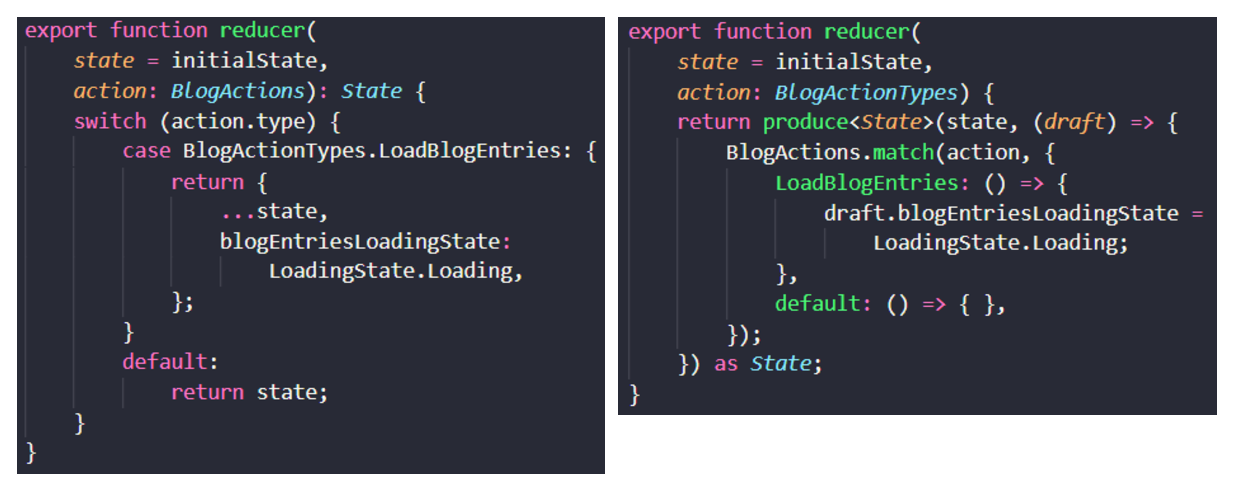
\includegraphics[width=1\linewidth]{PICs/with_and_without_immer_unionize_reducer.eps}
\caption{"BlogReducer" implemented without (left) and with the use of the methods "produce" and "match" from the JavaScript library Immer \cite{Immer} and the TypeScript library Unionize \cite{Unionize} (right).}\label{Fig5}
\end{figure}
Immer \cite{Immer} (removing some boilerplate code for writing reducers (produce)).
more features for reactive programming, Redux DevTools \cite{ReduxDevTools} as browser extension by importing the store devtools of ngrx into the AppModule.

\subsection{Adding a new Feature}
\begin{figure}[!htbp]
\centering
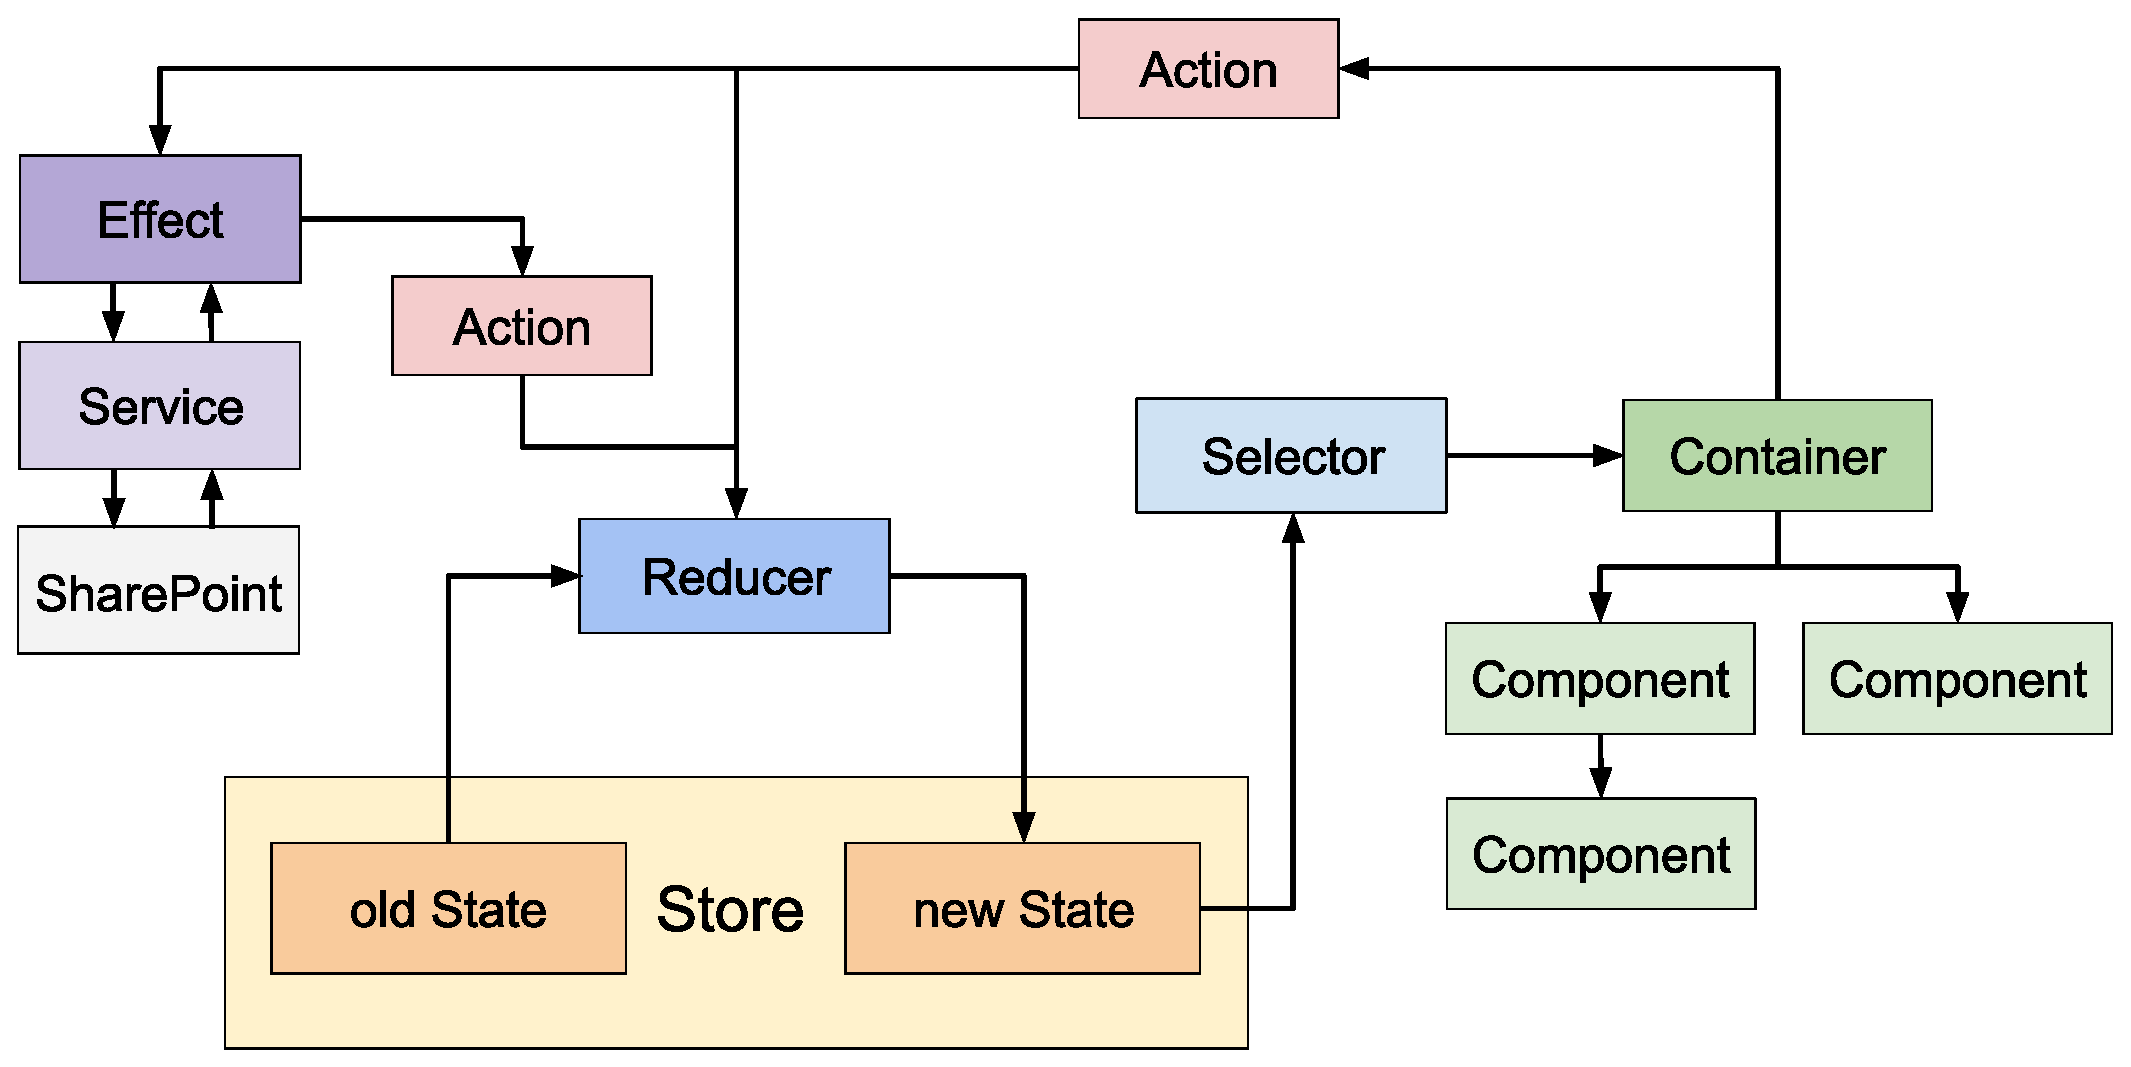
\includegraphics[width=0.75\linewidth]{PICs/ngrx_redux_structure.eps}
\caption{The Redux pattern in conjunction with NgRx}\label{Fig6}
\end{figure}
explain implementation in form of an example like "showing blog entry", Store, Actions, State, Reducer, Selector, Effect, etc., verweis auf \ref{Fig6}

\subsection{Unit Testing}
testing with reactive programming (reducer, effects (jasmine-marbles)); allgemein welche Technologien wurden genutzt: Karma \cite{Karma} (test runner; config for browser, reporters, frameworks, and more); Jasmine \cite{Jasmine} (behavior-driven development framework for testing); Karma-Mocha-Reporter \cite{KarmaMocha} (javascript test framework) and Karma-Jasmine-HTML-Reporter \cite{KarmaJasmineHTML} for reporting; Given-When-Then \cite{GivenWhenThen} format for structuring test cases; 

\clearpage


\chapter{Discussion}

\section{Development}
Difficulties (no need for PhantomJS anymore because of Chrome as headless browser), possible overhead of Redux huge advantages at a cost (also extensions for chrome which makes debugging less painful)

\section{Results}
presenting finished solution
\clearpage


\chapter{Conclusion \& Future Work}




% Hier beginnen die Verzeichnisse.
\clearpage
\ifthenelse{\equal{\FHTWCitationType}{HARVARD}}{}{\bibliographystyle{gerabbrv}}
\bibliography{Literatur}
\clearpage

% Das Abbildungsverzeichnis
\listoffigures
\clearpage

\listofcode
\clearpage

\phantomsection
\addcontentsline{toc}{chapter}{\listacroname}
\chapter*{\listacroname}
\begin{acronym}[XXXXX]
    \acro{API}[API]{Application Programming Interface}
    \acro{CLI}[CLI]{Command-Line Interface}
    \acro{CSS}[CSS]{Cascading Style Sheets}
    \acro{ECMA}[ECMA]{European Computer Manufacturers Association}
    \acro{HTML}[HTML]{Hypertext Markup Language}
    \acro{TFS}[TFS]{Team Foundation Server}
    \acro{UI}[UI]{User Interface}
    \acro{XML}[XML]{Extensible Markup Language}
\end{acronym}

\end{document}}